\documentclass{chi-ext}
% Please be sure that you have the dependencies (i.e., additional LaTeX packages) to compile this example.
% See http://personales.upv.es/luileito/chiext/

\copyrightinfo{
  Copyright is held by the author/owner(s).\\
  \emph{MobileHCI 2014}, September 23-26 2014, Toronto, Canada.\\
  ACM 978-1-XXXX-XXXX-X/XX/XX.\\
}

\title{Simple Visual and Vibrotactile Patterning within Wearable Mobile Gaming Experiences}

\numberofauthors{5}
% Notice how author names are alternately typesetted to appear ordered in 2-column format;
% i.e., the first 4 authors on the first column and the other 4 authors on the second column.
% Actually, it's up to you to strictly adhere to this author notation.
\author{
  \alignauthor{
  	\textbf{Adam Tindale}\\
  	\affaddr{OCAD University}\\
  	\affaddr{Toronto, ON M5T 1W1 Canada}\\
  	\email{atindale@faculty.ocadu.ca}
  }\alignauthor{
  	\textbf{Jessica Peter}\\
  	\affaddr{OCAD University}\\
  	\affaddr{Toronto, ON M5T 1W1 Canada}\\
  	\email{jp11jg@student.ocadu.ca}
  } 
    \vfil
  \alignauthor{
  	\textbf{Michael Cumming}\\
  	\affaddr{OCAD University}\\
  	\affaddr{Toronto, ON M5T 1W1 Canada}\\
  	\email{mcumming@ocadu.ca}
  }\alignauthor{
  	\textbf{Sara Diamond}\\
  	\affaddr{OCAD University}\\
  	\affaddr{Toronto, ON M5T 1W1 Canada}\\
  	\email{sdiamond@ocadu.ca}
  }
    \vfil
    \alignauthor{
  	\textbf{Hudson Pridham}\\
  	\affaddr{OCAD University}\\
  	\affaddr{Toronto, ON M5T 1W1 Canada}\\
  	\email{hp12pk@student.ocadu.ca}
  } 
}

% Paper metadata (use plain text, for PDF inclusion and later re-using, if desired)
\def\plaintitle{Simple Visual and Vibrotactile Patterning within Transmedia Gaming Experiences}
\def\plainauthor{Adam Tindale}
\def\plainkeywords{pattern recognition, wearable devices, gaming, multi-sensory, vibrotactile}
\def\plaingeneralterms{Gaming, Patterns, Wearable}

\hypersetup{
  % Your metadata go here
  pdftitle={\plaintitle},
  pdfauthor={\plainauthor},  
  pdfkeywords={\plainkeywords},
  pdfsubject={\plaingeneralterms},
  % Quick access to color overriding:
  citecolor=black,
  linkcolor=blue,
  menucolor=black,
  urlcolor=blue,
}

\usepackage{graphicx}   % for EPS use the graphics package instead
\usepackage{balance}    % useful for balancing the last columns
\usepackage{bibspacing} % save vertical space in references
\usepackage{paralist}

\begin{document}

\maketitle

\begin{abstract}
Simple, wearable devices are a promising way of encouraging participation with those who consume, and contribute to, media. In this paper we explore techniques for adding simple visual and vibro-tactile patterning for children aged 8-12, which add sensory interest to gameplay as well as convey useful information about basic game dynamics and expected user interactions. In this paper we describe a series of demo experiences focusing on the communication of information through low resolution vibrotactile and LED displays.
\end{abstract}

\keywords{\plainkeywords}

\category{H.5.2}{Information interfaces and presentation (e.g., HCI)}{User Interfaces}. 

\terms{\plaingeneralterms}


% ===========================================================================
\section{Introduction}
% ===========================================================================

Gaming controllers provide users with the opportunity to expertly control a game experience. However, game controllers are purpose driven devices that provide little utility when not conneted to the game experience. While there have been many interesting uses of game controllers outside of game experiences, the controllers themselves rely on being attached to hardware in order to have any function. Instead, we take a different approach: we try to make the interactions very simple, such that they convey information in a way that presents few cognitive demands on the user and which the user would tend to find enjoyable and engaging even if they were not participating in a mobile game. 

Our demo experiences focus on an attempt to make the interactions very simple, such that they convey information in a way that presents few cognitive demands on the user and which the user would tend to find enjoyable and engaging, even if they were not participating in a mobile game. 


If well done they engage viewers and can build interesting, emergent social cohorts. They have the potential of explaining and making connections between complex concepts in a fluid and graceful way. However, because of this fluidity of structure they demand a high level of skill in their artistic conception and organization. 


The basic device use cases that might inform the gamer during gameplay, which also could apply to a viewer navigating through a narrative, are: 
\begin{inparaenum}[\itshape a\upshape)]
  \item what is my current position or state within the game?
  \item do I need to make any decisions or choices in order to proceed with the game?
  \item is anything else happening in the game of which I should be aware? and,
  \item what comes next in the game? 
\end{inparaenum}

In addition to the gaming or narrative aspects, within social transmedia games such as Time Tremors there are also social interactions with other gamers in which gameplay is influenced greatly by the actions of others. 

Time Tremors is also a collections-type game in which gamers collect items of value both within the game and also by getting items from other gamers. 

For the social and collection aspects of a game like Time Tremors we have identified several important use cases: 
\begin{inparaenum}[\itshape a\upshape)]
\item detect other band wearers (wirelessly) who happen to be in the vicinity
\item give something of value to another wearer, 
\item exchange something of value with another wearer, and
\item give the wearer some indication of the game mode the wearer is in.
\end{inparaenum}

Therefore, in Time Tremors type games, which is typical of transmedia game in general, many things are going on simultaneously: there is complex navigation through a graph of narrative possibilities, there are social interactions within other gamers also experiencing related narratives in their own way, and finally there is a artefact-based collection aspect in which items of value are collected and exchanged between gamers. 

Such complexity could easily get out of hand. Instead, our goal is to create integrated user experiences that are simple and enjoyable. Our goal is despite how complex the game mechanics might be the device and how to use it remain relatively simple and straightforward.

Our demo experiences focus on an attempt to make the interactions very simple, such that they convey information in a way that presents few cognitive demands on the user and which the user would tend to find enjoyable and engaging.

% ======================================================================
\section{Related Work}
% ======================================================================

Ruspini provides a useful introduction to the concepts and history of haptics, the basics of haptic psychophysics and haptic devices past and present \cite{ruspini1999haptics}.

MacLean \cite{maclean2009putting} discusses the potential benefits of haptic feedback as an ambient notification system. Unlike visual information, which can be obtrusive while completing a task, or sound, which can be obnoxious in a public environment, haptic feedback is usually experienced only by the user and does not directly interfere with the task at hand. 

In Profita (2013) \cite{profita2013don} researchers reveal the results of studies completed in the United States and South Korea on the social acceptability of interacting with on-body controllers in which participants  ranked factors such as ?awkwardness? and ?coolness? of the exhibited interactions as actors performed them. This article is helpful for providing insight on social acceptability of wearable positioning as it relates to gender and culture.

Oliveira and Maciel propose a network of haptic actuators that use a set of patterns to express elements of an environment that has obstacles and free paths and demonstrates the use of a haptic language that helps users navigate and consists of vibrotactile signs to complement or replace their vision. \cite{Jesus-Oliveira:2013aa}

De Jesus Oliveira and Maciel \cite{Jesus-Oliveira:2013aa} present research towards building a hand-mounted array of haptic actuators intended to help the wearer perform a variety of tasks including orientation. They propose that the actuators could be connected to environment-aware sensors so that the actuators would vibrate in a set pattern to alert the wearer of an obstacle (or help instruct them to perform a certain task). Such haptic systems could help visually impaired users navigate. They would also enable fully sighted users to perform certain tasks without being distracted by personal technologies (i.e. using a smartphone to check a map).


% ======================================================================
\section{Prototypes and Case Studies}
% ======================================================================

Prototypes began as the simplest and least refined expression of a wearable or functional haptic device. The first prototype has simple linear arrangement of LED light and mobile phone type vibrating motors. When the connected to an Arduino micro-controller this band emits a rhythmic and visual sequential pattern that could conceivably could be used to notify band wearers of others in their vicinity. Although this band was perhaps the most simplistic band possible, it could in fact be functional in some minimal sense for a transmedia gaming experience. Also, such a minimal band would be inexpensive to manufacture and simple to program. 



\begin{figure}
  \begin{center}
  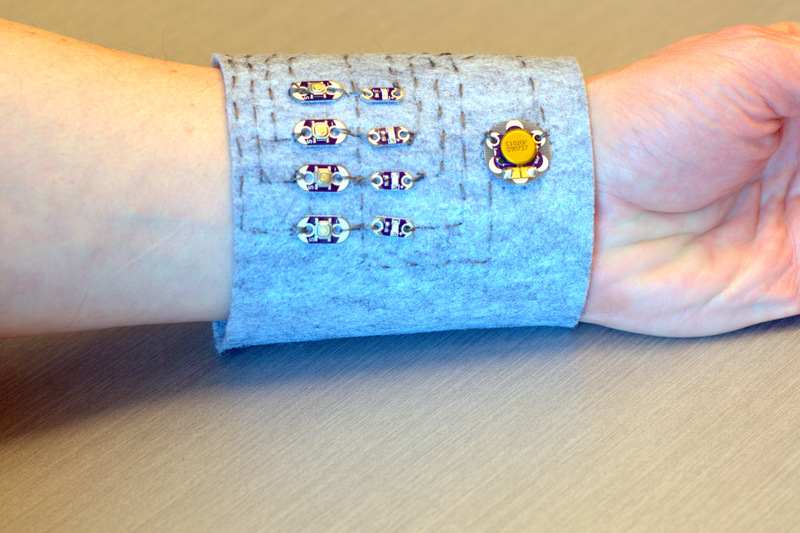
\includegraphics[width=\columnwidth]{images/P1130375.jpg}
  \caption{A wearable version of the traditional simon says game. The LEDs flash in a random pattern. The wearer must repeat the pattern flashed by the LEDs by pressing the buttons directly adjacent to each LED.}
  \label{fig:marginparsample}
  \end{center}  
\end{figure}

\begin{figure}
  \begin{center}
  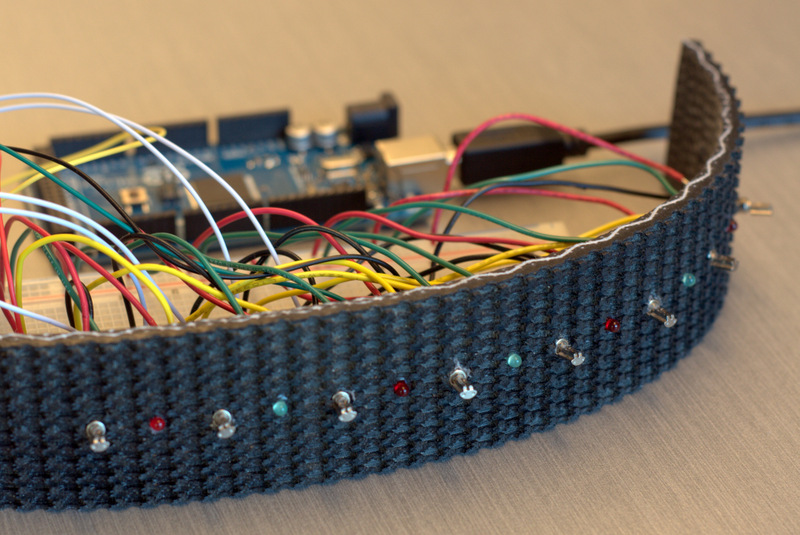
\includegraphics[width=\columnwidth]{images/P1130386.jpg}
  \caption{A simple prototype that features visual and vibrotactile sensory outputs.}
  \label{fig:rubberVibeBand01}
  \end{center}  
\end{figure}

\section{Discussion and Conclusions}

This paper has demonstrated a number of interfaces that provide wrist based vibrotactile displays. Our work has shown that providing a vibrotactile array instead of a simple vibration motor provides user with a many more pathways of recieving and perceiving information.

%\section{Future Work}
%Wearable devices and associated technologies for developing is developing at a rapid pace.
%Miniaturization, bearability and functionality is obviously a primary concern of such devices. 

\section{Acknowledgements}
%We thank the valuable input from Patrick Crowe and all those at Xenophile Media Inc. who have great expertise in crafting transmedia narratives; Dr. Rachel Zuannon from the Graduate Design Program at Anhembi Morumbi University, Sao Paulo, Brazil.; the professors, students and staff within OCAD University's Digital Futures Initiative (DFI) for their valuable input and helpful comments. The following students within the DFI program worked on this project over many months: Hudson Pridham, Ryan Maksymic, Jessica Peter and Boris Kourtoukov. We thank Dr. Steve Szigeti for his contributions to this project and we especially thank Dr. Sara Diamond, President of OCAD University for her guidance and support.

We would like to thank Ryan Maksymic, Boris Kourtoukov, and Steve Szigeti for their help in the development of this project. This work is generously supported by grants from the Natural Sciences and Engineering Research Council of Canada (NSERC), International Science and Technology Partnerships Canada.

\balance
\bibliographystyle{acm-sigchi}
\bibliography{MGDSPET}

\end{document}
